%! TeX program = lualatex
\documentclass[../main.tex]{subfiles}
\begin{document} \section{Applied optimization problems}
  To optimize is to find the absolute maximum or absolute minimum of some function. The mathematical idea of modern machine learning (or AI) is to find a function (given some known data set) that \emph{minimizes} certain type of error measurement. The resulting function is used to \emph{predict} the future.

  Optimization problems are good opportunities to work on our problem-solving skills. A combination of geometry, algebra skills and differential calculus usually go into solving an optimization problem.

  Here re the big ideas.
  \begin{enumerate}[label=(\alph*)]
    \item We know how to find absolute extrema (or values at which absolute extrema occur) of functions in a \hlmain{single} variable.

    \item However, it is often easier to \hlmain{describe} real-world science problems using more than one variables.

    \item We need to use our algebra skill to transform a multi-variable problem to an equivalent single-variable problem.

    \item Finally, we use calculus to solve a problem in a single variable.
  \end{enumerate}


  \textbf{The general optimization strategy}
  \label{page:optimization-strategy}
  \begin{enumerate}[label=(\arabic*)]
    \item Sketch the given scenario and \emph{introduce variables}. Make sure every variable measures something.

    \item Identify the \hlwarn{objective variable}. Write one of the following
      \begin{itemize}
        \item \emph{\hlattn{Goal: We want to minimize/maximize \ldots{}.}}
        \item \emph{\hlattn{Goal: We want to find \ldots{} at which \ldots{} occurs.}}
      \end{itemize}

    \item Use the given scenario and our sketch to figure out the \hlmain{relation} among our variables. Write down function(s), equation(s) and whatever it takes to fully describe the scenario in mathematical terms. We typically end up with one or more equations. 

    \item Treat the objective variable as the dependent variable and all other variables as independent. Eliminate all but one independent variable, so that the objective variable is a single-variable function in the remaining variable.

      \hlsupp{Common misadventures at this step?}
      \begin{itemize}
        \item If we cannot eliminate all but one independent variable, then maybe modify our description in Step~(1) or find hidden relations in Step~(3).
        \item Algebra mistakes can also happen here.
        \item Sometimes, especially when we are stressed or under time pressure, we eliminate the objective variable away. That's why step (2) is important. Always make sure we know what the goal is.
      \end{itemize}

    \item \hlattn{Achieve the goal we wrote down in step (2)} using techniques from previous sections (finding absolute extrema, derivative tests, asymptotes, and/or basic algebra).

  \end{enumerate}
  \clearpage

  Let's start with a warm-up example to get the big picture. As usual, we introduce problem-solving strategies within an example. The full strategy is on page~\pageref{page:optimization-strategy}.
  \begin{example} \label{ex:optimization-fence}
    We have \(100\) metres of fence material and want to enclose a rectangular area with one side against the wall. The interior is \emph{evenly} divided into two divisions by putting up a fence parallel to the sides perpendicular to the wall. What is the largest area we can enclose?

    \begin{enumerate}[wide, noitemsep]
      \item Sketch the given scenario and \emph{introduce variables}. Make sure every variable measures something.
        \blanklines{5}

      \item Identify the \hlwarn{objective variable}. Write ``\emph{\hlattn{Goal: We want to minimize/maximize \ldots{}}}.''
        \blanklines{3}

      \item Use the given scenario and our sketch to figure out the \hlmain{relation} among our variables. 
        \blanklines{5}

      \item Eliminate all but one independent variable, so that the objective variable is a single-variable function in the remaining independent variable. \hlinfo{Also figure out the domain of the resulting function using the given scenario.}
        \blanklines{10}

      \item \hlattn{Achieve the goal we wrote down in step (2)} using techniques from previous sections.
        \blanklines{10}
    \end{enumerate}
  \end{example}
  \clearpage

  Example~\ref{ex:optimization-swim} is a slight variation of Example~\ref{ex:optimization-fence} where the \emph{obvious} (depends on the person) description of a given problem results in hidden information. Develop algebra and geometry skills to uncover potentially hidden information (mathematical relations). Hint: If you have \(n\) independent variables, then you should have at least \(n\) equations in Step~(3).

  \begin{example} \label{ex:optimization-swim}
    A  river is \(1\) km wide. You are standing on the bank of the river and want to reach the opposite side, \(2\) km down the river. You can swim \(3\) kph (kilometres per hour) and walk \(6\) kph. Minimize your travel time.

    \hfill{}
    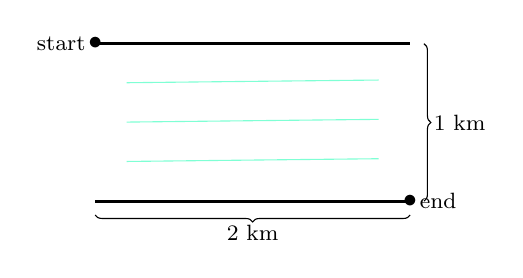
\begin{tikzpicture}[scale=2]
      \node at (0,1) {\(\bullet\)};
      \node[left] at (0,1) {\footnotesize start};
      \node at (2,0) {\(\bullet\)};
      \node[right] at (2,0) {\footnotesize end};
      \draw[very thick] (0,0) -- (2,0);
      \draw[very thick] (0,1) -- (2,1);
      \draw[decorate, decoration={brace, raise=5pt}] (2,0) -- (0,0)
        node[midway, below=5pt] {\footnotesize \(2\) km};
      \draw[decorate, decoration={brace, raise=5pt, mirror}] (2,0) -- (2,1)
        node[midway, right=5pt] {\footnotesize \(1\) km};
      \draw[Aquamarine, domain=0.2:1.8, smooth, samples=100] plot ({\x},{sin(4*pi*\x)*0.05+0.75});
      \draw[Aquamarine, domain=0.2:1.8, smooth, samples=100] plot ({\x},{sin(4*pi*\x)*0.051+0.50});
      \draw[Aquamarine, domain=0.2:1.8, smooth, samples=100] plot ({\x},{sin(4*pi*\x)*0.051+0.25});
    \end{tikzpicture}

    \begin{enumerate}[wide, noitemsep]
      \item The sketch is given. Introduce variable(s) to describe the scenario.
        \blanklines{4}

      \item Identify the \hlwarn{objective variable}. Write ``\hlattn{Goal: We want to maximize/minimize \ldots{}}''. 
        \blanklines{3}

      \item Figure out the relations among our variables. If we have \(n\) independent variables, then we should have at least \(n\) equations.
        \blanklines{8}

      \item Eliminate all but one independent variable, so that the objective variable is a single variable function in the remaining independent variable. Also figure out the domain of the resulting function using the given scenario.
        \blanklines{10}

        \vfill{}{\footnotesize (continues onto the next page)} \clearpage

      \item \hlattn{Achieve the goal we wrote down in Step (2)}. Be very clear of the mathematical problem we are about to solve.
        \blanklines{15}
    \end{enumerate}
  \end{example}

  \medskip
  Example~\ref{ex:optimization-closest-point-to-curve} demonstrates an application of optimization techniques to \hlattn{find value(s) at which} the absolute minimum/maximum \hlattn{occur(s)}. In such problems, we don't really care about the actual absolute extrema value. 

  \begin{example} \label{ex:optimization-closest-point-to-curve}
    Find the point on the ellipse \(4x^{2} + y^{2} = 4\) that is closest to the point \(A = (1,-2)\). Take for granted that such point exists.

    \begin{enumerate}[wide, noitemsep]
      \item Sketch the given scenario and \emph{introduce variables}. Make sure every variable measures something. 
        \blanklines{5}

      \item This question does not directly ask us to maximize/minimize something. Rather, it asks us to find \underline{\hspace{1in}} at which \underline{\hspace{2in}}. \url{https://www.geogebra.org/calculator/rkxfbt3z}

        Identify the \hlwarn{objective variable}. Write ``\emph{\hlattn{Goal: We want to find \ldots}}.''
        \blanklines{3}

      \item Figure out the relations among our variables. 
        \blanklines{10}

        \vfill{}{\footnotesize (continues onto the next page)} \clearpage

      \item Eliminate all but one independent variable, so that the objective variable is a single-variable function in the remaining independent variable. 
        \blanklines{10}

      \item \hlattn{Achieve the goal we wrote down in Step (2)}. Remember we have to find the associated \((x,y)\) values as well. 

        Computational shortcut: Minimizing \(d\) is the same as minimizing \(d^{2}\).
        \blanklines{30}
    \end{enumerate}
  \end{example}
  \clearpage

  \clearpage

  \begin{example} \label{ex:optimization-ladder}
    Suppose a \(2\)-metre tall fence stands \(1\) metre away from a tall wall.  What is the shortest ladder that will reach over the fence to the wall.
    \blanklines{54}
  \end{example}

  \begin{example}
    A haunted house is trying to maximize revenue for next year. This year, if the ticket price was \textdollar{20}, then the average attendance was \(500\) visitors per evening. If the ticket price was \textdollar{15}, then the average attendance was \(800\) visitors per evening.  Assume average visitor per evening is linearly related to ticket price.

    Find the ticket price that maximizes revenue per evening. 
    \blanklines{49}
  \end{example}

  \begin{example}
    Take a standard printer paper which has dimension \(8.5 \times 11\) inches. We want to fold it down the middle of the long side (and parallel to the short side) to create a prism shape. Assume the two ends of the prism are sealed. What is the angle between the two folded sides that maximizes the volume of the resulting prism?

    \blanklines{45}

    \faComment{} What if the paper has dimension \(1094379843 \times 43286493247839274932\) inches?? What angle maximizes the volume? Does the dimension of the paper matter at all?
  \end{example}

\end{document}
